\section{CQ8}

\begin{fancyquote}
    \textbf{Question:}\\
    Compare the local broker usage in the two capture files \texttt{A.pcapng} and \texttt{B.pcapng}. The goal is to have a plot on the number of layers of the topics used in the publish messages directed to the local broker in the two captures.
\end{fancyquote}

For this question, we considered only MQTT \texttt{PUBLISH} messages \textbf{directed to the local broker}, i.e.\ messages entering the broker, and not messages sent by the broker to subscribers.

\subsection*{Dataset A}

First, we identified the local broker in \texttt{A.pcapng} by inspecting MQTT \texttt{CONNECT} packets. The relevant connections were directed to \texttt{127.0.0.1:1883}, so the local broker is the loopback broker.

To extract only MQTT \texttt{PUBLISH} packets entering the local broker, we used:

\begin{lstlisting}
tshark -r A.pcapng -Y "mqtt.msgtype == 3 && tcp.dstport == 1883 && ip.dst == 127.0.0.1" -T fields -e frame.number -e tcp.stream -e tcp.srcport -e tcp.dstport -e mqtt.topic > A_publish_into_broker_port1883.txt
\end{lstlisting}

The total number of considered publish messages is obtained with:

\begin{lstlisting}
wc -l < A_publish_into_broker_port1883.txt
\end{lstlisting}

which gives:

\begin{verbatim}
439
\end{verbatim}

Then we computed the number of topic layers by splitting each topic on the \texttt{/} character:

\begin{lstlisting}
awk -F '\t' '{
    topic=$5;
    n=split(topic,a,"/");
    print n
}' A_publish_into_broker_port1883.txt | sort -n | uniq -c
\end{lstlisting}

This produced:

\begin{verbatim}
154 2
131 3
154 4
\end{verbatim}

So for \texttt{A.pcapng}:
\begin{itemize}
    \item Layer 1: 0
    \item Layer 2: 154
    \item Layer 3: 131
    \item Layer 4: 154
\end{itemize}

\subsection*{Dataset B}

For \texttt{B.pcapng}, we first extracted all MQTT \texttt{PUBLISH} messages directed to brokers on port \texttt{1883}:

\begin{lstlisting}
tshark -r B.pcapng -Y "mqtt.msgtype == 3 && tcp.dstport == 1883" -T fields -e frame.number -e ip.src -e ip.dst -e tcp.srcport -e tcp.dstport -e mqtt.topic > B_publish_to_brokers.txt
\end{lstlisting}

By checking the IPv4 and IPv6 destination fields, we observed that the local broker traffic appears on loopback IPv6 (\texttt{::1}), while the public HiveMQ traffic uses external IPv4 addresses. In the original extraction, these loopback IPv6 packets appeared with an empty \texttt{ip.dst} field. Therefore, we isolated local broker publish traffic with:

\begin{lstlisting}
awk -F '\t' '$3 == "" {print}' B_publish_to_brokers.txt > B_local_publish.txt
\end{lstlisting}

The total number of considered publish messages is:

\begin{lstlisting}
wc -l < B_local_publish.txt
\end{lstlisting}

which gives:

\begin{verbatim}
534
\end{verbatim}

Then we computed the number of topic layers with:

\begin{lstlisting}
awk -F '\t' '{
    topic=$6;
    n=split(topic,a,"/");
    print n
}' B_local_publish.txt | sort -n | uniq -c
\end{lstlisting}

This produced:

\begin{verbatim}
21  1
172 2
162 3
179 4
\end{verbatim}

So for \texttt{B.pcapng}:
\begin{itemize}
    \item Layer 1: 21
    \item Layer 2: 172
    \item Layer 3: 162
    \item Layer 4: 179
\end{itemize}

\subsection*{Final result}

The final topic-layer distributions are:

\begin{center}
\begin{tabular}{c|cc}
\textbf{Number of layers} & \textbf{Dataset A} & \textbf{Dataset B} \\
\hline
1 & 0   & 21  \\
2 & 154 & 172 \\
3 & 131 & 162 \\
4 & 154 & 179 \\
\end{tabular}
\end{center}

\begin{figure}[H]
    \centering
    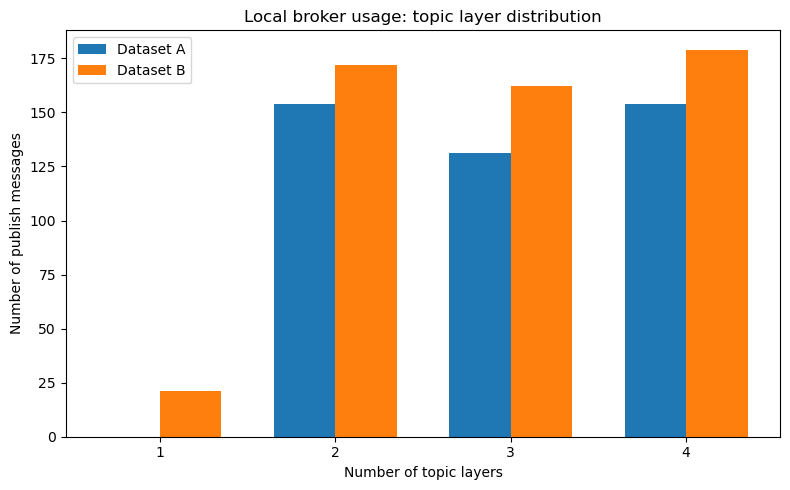
\includegraphics[width=0.75\linewidth]{images/cq8_plot.png}
    \caption{Histogram of the number of topic layers in MQTT \texttt{PUBLISH} messages directed to the local broker, comparing \texttt{A.pcapng} and \texttt{B.pcapng}.}
\end{figure}

The total number of publish messages considered for the analysis is:

\begin{itemize}
    \item \texttt{A.pcapng}: 439
    \item \texttt{B.pcapng}: 534
\end{itemize}

Therefore:

\vspace{0.3cm}

\noindent{\huge\bfseries Answer CQ8a: 439\par}

\vspace{0.3cm}

\noindent{\huge\bfseries Answer CQ8b: 534\par}